\documentclass {article}

\usepackage[utf8]{inputenc}
\usepackage[english,greek]{babel}
\usepackage{alphabeta}
\usepackage[T1,LGR]{fontenc}

% For more math mode styles
\usepackage{amsmath}

% For images
\usepackage{graphicx}

% For more colors
\usepackage{color}

% Drawing diagrams
\usepackage{tikz}

% Octave code highlighting
\usepackage{listings}

% Links
\usepackage{hyperref}

%% Options

% For hyperlinks
\hypersetup{
	colorlinks=true,
	linkcolor=blue,
	filecolor=magenta,      
	urlcolor=cyan,
}

\urlstyle{same}

% Colors
\definecolor{codegreen}{rgb}{0,0.6,0}
\definecolor{codegray}{rgb}{0.5,0.5,0.5}
\definecolor{codepurple}{rgb}{0.58,0,0.82}
\definecolor{backcolour}{rgb}{0.95,0.95,0.92}
 
% Listing Style
\lstdefinestyle{mystyle}{
	backgroundcolor=\color{backcolour},
    commentstyle=\color{codegreen},
    keywordstyle=\color{magenta},
    numberstyle=\tiny\color{codegray},
    stringstyle=\color{codepurple},
    basicstyle=\scriptsize\ttfamily,
    breakatwhitespace=false,         
    breaklines=true,                 
    captionpos=b,                    
    keepspaces=true,                 
    numbers=left,                    
    numbersep=5pt,                  
    showspaces=false,                
    showstringspaces=false,
    showtabs=false,                  
    tabsize=4
}

\lstset{style=mystyle}

%Tikz options
\usetikzlibrary{fadings}
\usetikzlibrary{backgrounds}
\usetikzlibrary{arrows}
\usetikzlibrary{shapes,shapes.geometric,shapes.misc}

% this style is applied by default to any tikzpicture included via \tikzfig
\tikzstyle{tikzfig}=[baseline=-0.25em,scale=0.5]

% these are dummy properties used by TikZiT, but ignored by LaTex
\pgfkeys{/tikz/tikzit fill/.initial=0}
\pgfkeys{/tikz/tikzit draw/.initial=0}
\pgfkeys{/tikz/tikzit shape/.initial=0}
\pgfkeys{/tikz/tikzit category/.initial=0}

% standard layers used in .tikz files
\pgfdeclarelayer{edgelayer}
\pgfdeclarelayer{nodelayer}
\pgfsetlayers{background,edgelayer,nodelayer,main}

% style for blank nodes
\tikzstyle{none}=[inner sep=0mm]

% Images folder
\graphicspath{{./images/}}

% Paragraph options 
\setlength{\parskip}{\baselineskip}%
\setlength{\parindent}{0pt}%

% Writing in English command
\newcommand{\english}[1]{\foreignlanguage{english}{#1}}

\title{3\textsuperscript{ή} Εργαστηριακή Άσκηση στο μάθημα
Συστήματα Αναμονής}

\author{Λεωνίδας Αβδελάς $|$ AM: 03113182} 

\date{}

\begin{document}

\pagenumbering{gobble}

\maketitle

\pagenumbering{arabic}

\section*{Προσομοίωση συστήματος Μ/Μ/1/10}

Σχεδιάσαμε και υλοποιήσαμε την προσομοίωση του συστήματος σε \english{Octave}. Σχεδιαστικά βασιστήκαμε στον κώδικα που μας δόθηκε από το εργαστήριο. Η αλλαγή που κάναμε ήταν ότι μετά τις 10 καταστάσεις, ουσιαστικά θεωρούσαμε ότι το $λ = 0$ και άρα δεν υπήρχε πιθανότητα για περαιτέρω μετάβαση. 

\subsection*{(1)}

Εξετάσαμε τα αποτελέσματα για τα πρώτα 30 βήματα της προσομοίωσης και εξακριβώσαμε ότι όντως δούλευε με τον αναμενόμενο τρόπο.

\subsection*{(2)}

Στο Σχήμα \ref{fig:lambda-1}, βλέπουμε τα αποτελέσματα της προσομοίωσης για $λ=1$. Στο Σχήμα \ref{fig:lambda-5}, βλέπουμε τα αποτελέσματα της προσομοίωσης για $λ=5$. Στο Σχήμα \ref{fig:lambda-10}, βλέπουμε τα αποτελέσματα της προσομοίωσης για $λ=10$. Όλες οι προσομοιώσεις έχουν την ίδια σειρά ψευδό-τυχαίων αριθμών. Όπως βλέπουμε, για $λ=10$, το σύστημα βρίσκεται πάντα στην κατάσταση 10, δηλαδή είναι γεμάτο, οπότε δεν μπορεί να υπάρξει άλλη άφιξη.
Για $λ=5$, έχουμε ισορροπία στο σύστημα, και μικρότερη πιθανότητα απόρριψης.


\begin{figure}
    \centering
    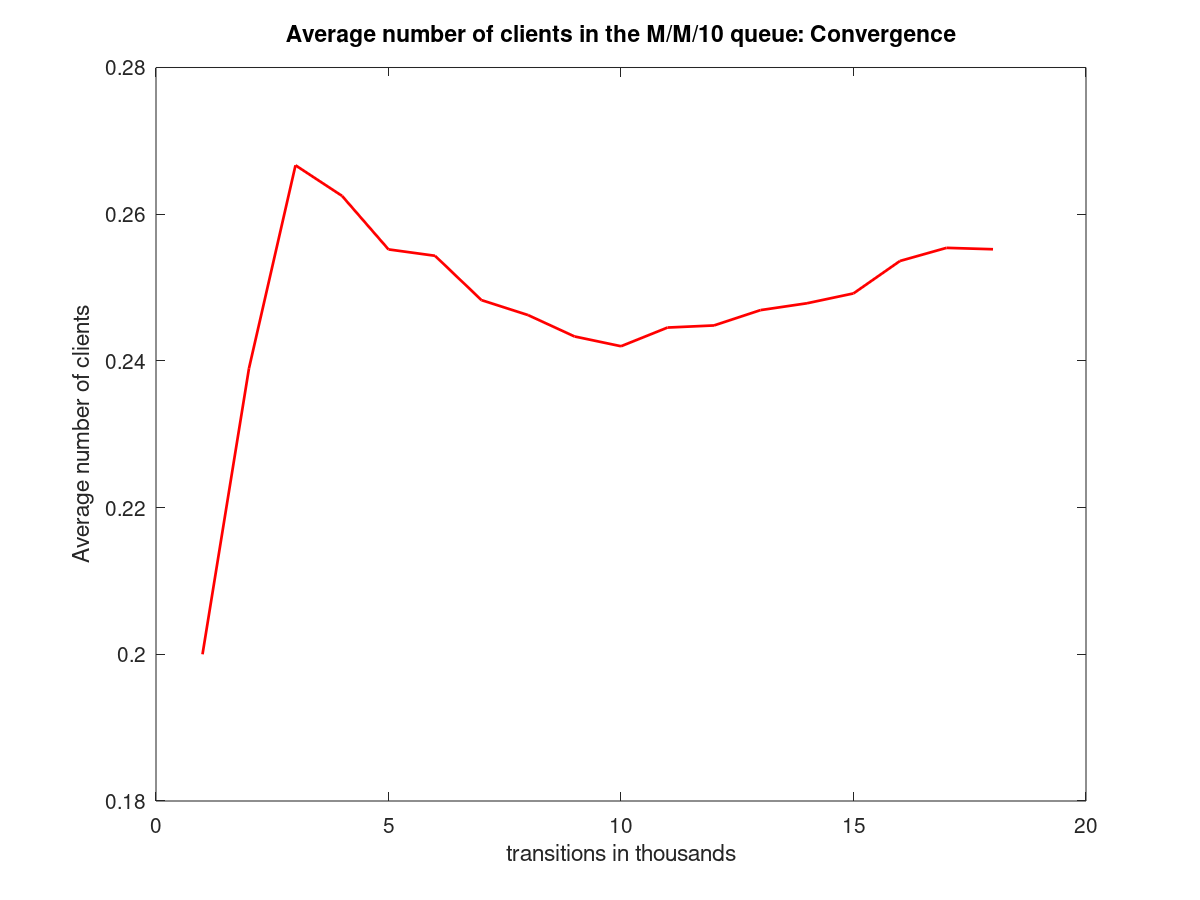
\includegraphics[width=0.5\textwidth]{lambda-1-average-clients.png}\hfill
    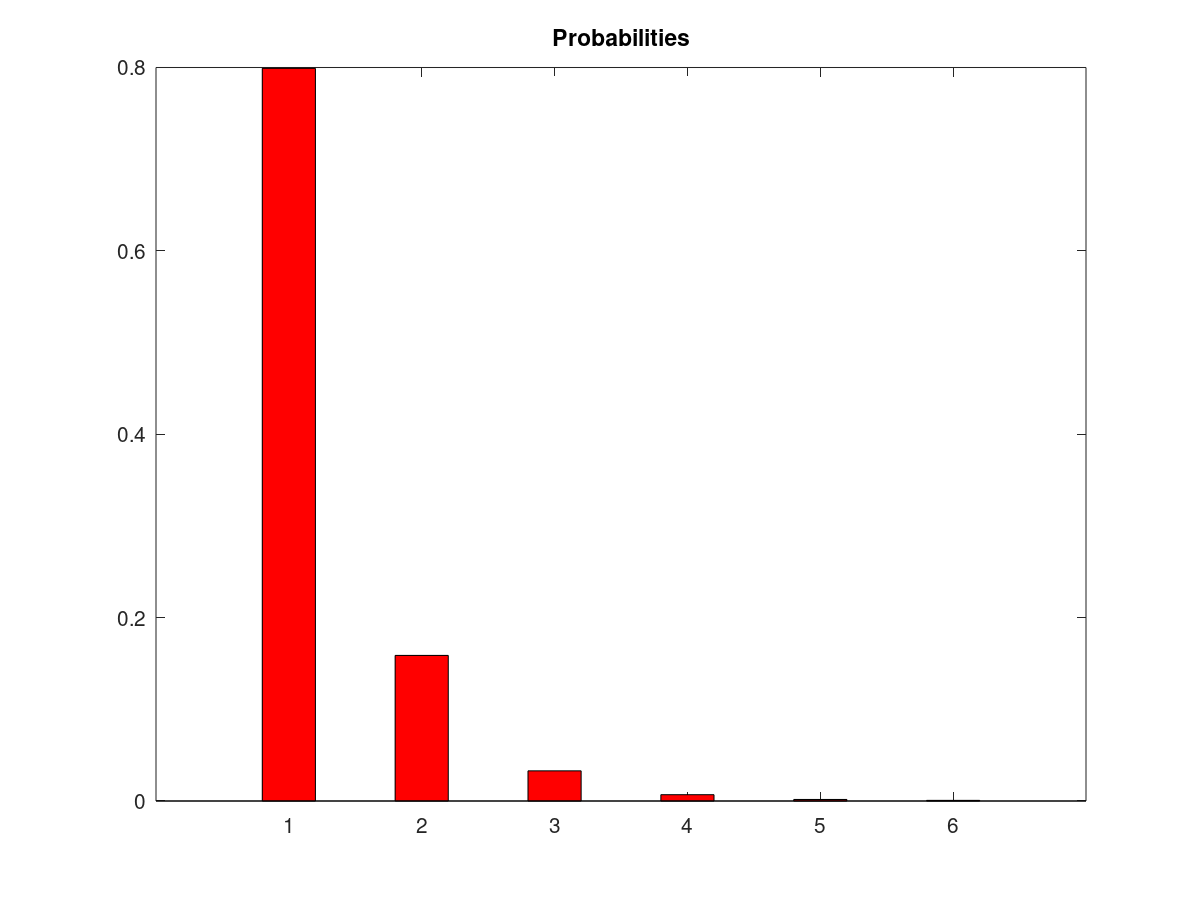
\includegraphics[width=0.5\textwidth]{lambda-1-probs.png}\hfill
    \caption{Προσομοίωση για $λ=1$}
    \label{fig:lambda-1}
\end{figure}

\begin{figure}
    \centering
    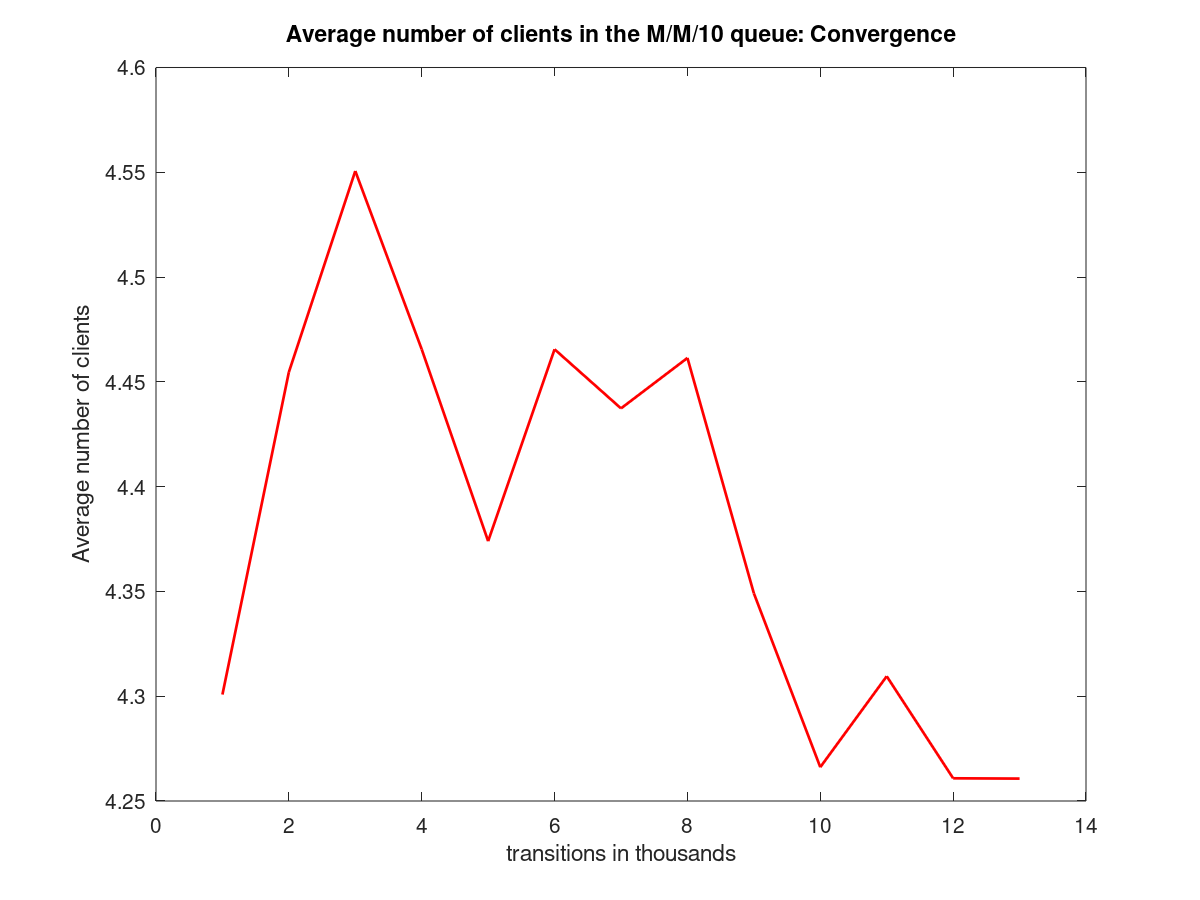
\includegraphics[width=0.5\textwidth]{lambda-5-average-clients.png}\hfill
    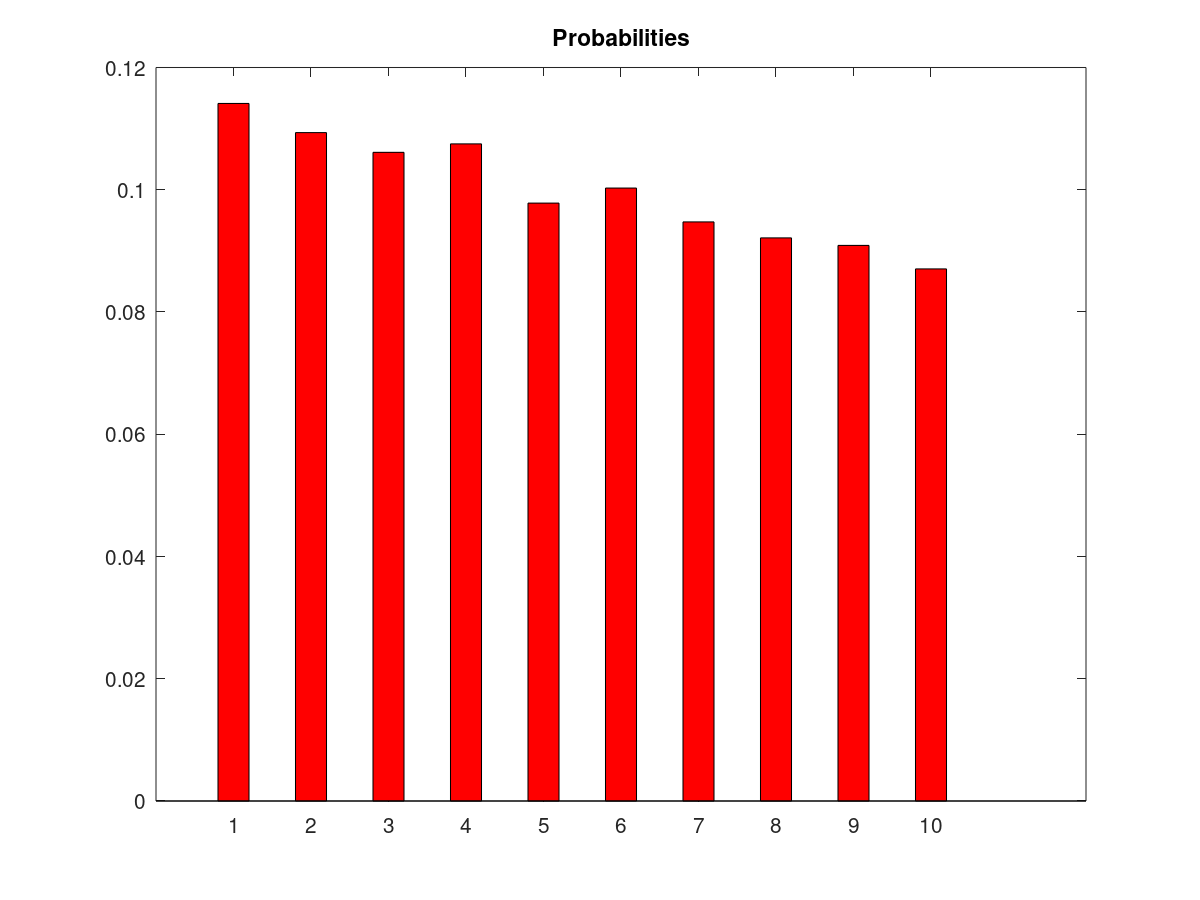
\includegraphics[width=0.5\textwidth]{lambda-5-probs.png}\hfill
    \caption{Προσομοίωση για $λ=5$}
    \label{fig:lambda-5}
\end{figure}

\begin{figure}
    \centering
    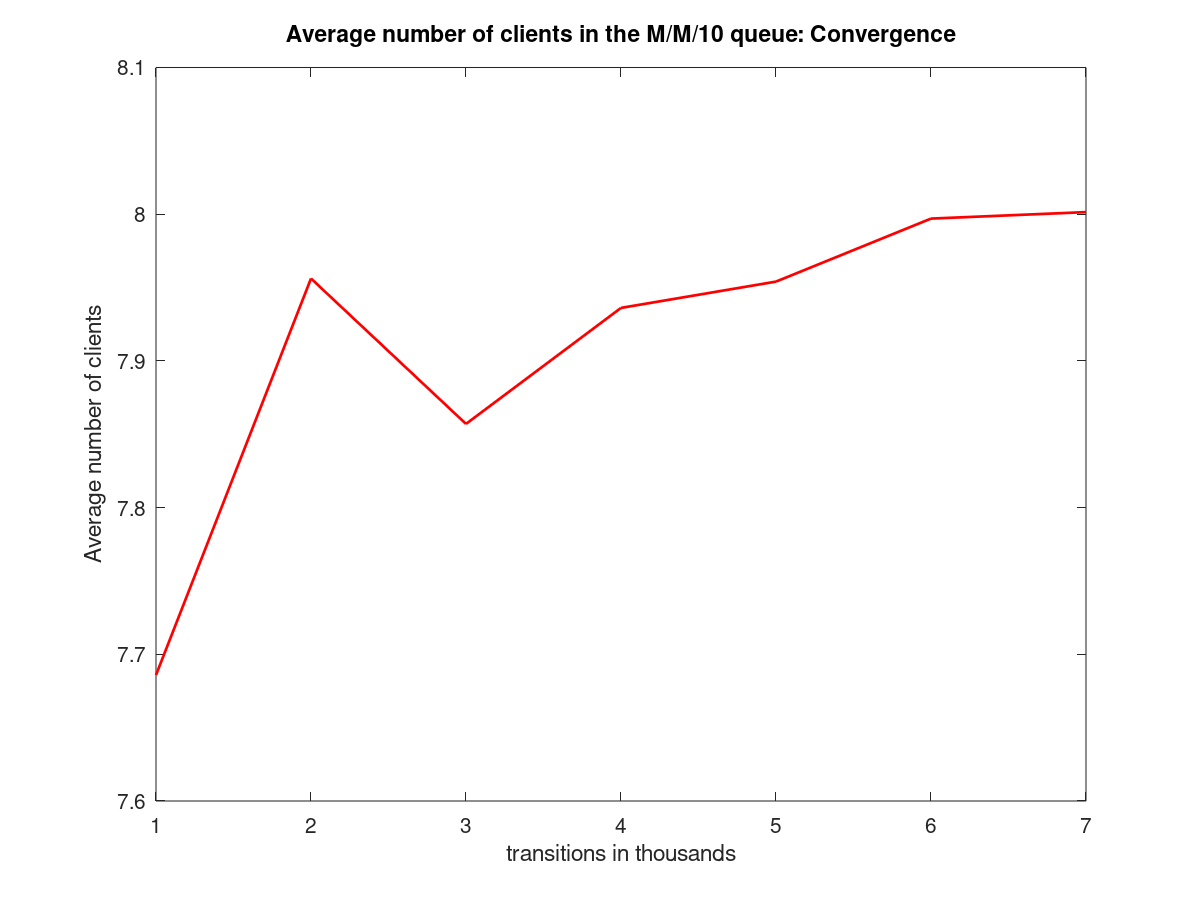
\includegraphics[width=0.5\textwidth]{lambda-10-average-clients.png}\hfill
    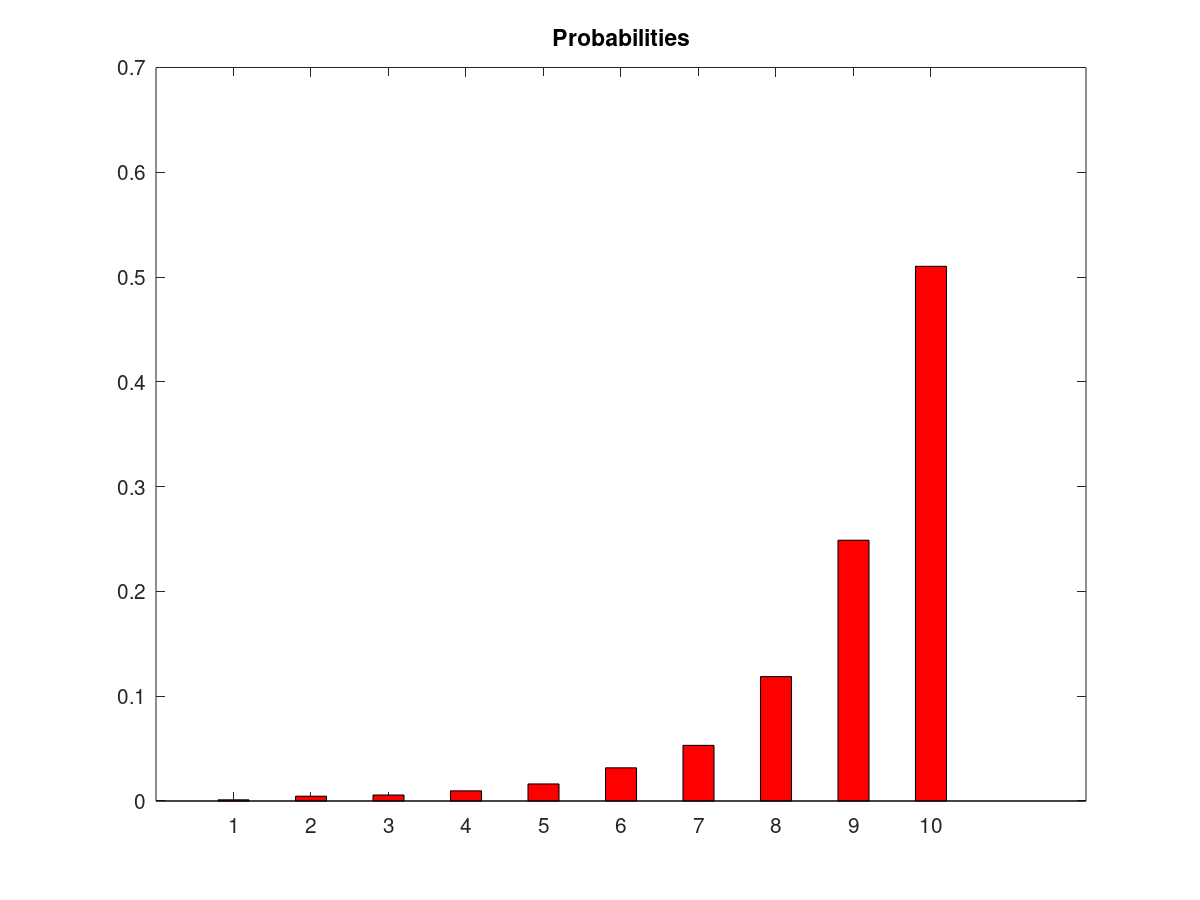
\includegraphics[width=0.5\textwidth]{lambda-10-probs.png}\hfill
    \caption{Προσομοίωση για $λ=10$}
    \label{fig:lambda-10}
\end{figure}

\subsection*{(3)}

Η ταχύτητα σύγκλισης φαίνεται να μικραίνει όσο μεγαλώνει το $λ$. Παρόλα αυτά βλέπουμε ότι το διάστημα στο οποίο κινήται ο μέσος αριθμός πελατών, μεγαλώνει όσο μεγαλώνει το $λ$. 

Έτσι, για $λ=1$, μετά τις πρώτες $5000$ μεταβάσεις, οι τιμές φαίνονται αρκετά σταθερές. Για $λ=5$, το σημείο αυτό είναι μετά από $8000$ μεταβάσεις. Για $λ=10$, μετά από περίπου $6000$ μεταβάσεις. Έτσι συνολικά, μετά από περίπου $6000$ θα έχουμε φτάσει στην σταθερή κατάσταση.

\subsection*{(4)}
Η αλλαγή θα ήταν αρκετά εύκολη, αφού απλά θα ορίζαμε το $μ$ ώς συνάρτηση της τρέχουσας κατάστασης σε κάθε μετάβαση. Επίσης το \english{threshold} θα έπρεπε να υπολογίζεται από την αρχή κάθε φορά.


\section*{Παράρτημα: Κώδικας \english{Octave}}

\selectlanguage{english}
\lstinputlisting[language=Octave]{finite_storage.m}


\lstinputlisting[language=Octave]{lab3.m}

\end{document}